\chapter{Literature Survey}

This section will be explained why there’s a need for this system by explore background literature relate to this subject. Mainly the need of a proper system to test scientific software, start with explaining what a scientific software is, following up by explain why most of are not tested correctly. Then we will be discussing the two main component of this system, cucumber and behave. Then finally, explaining what casual testing is, the main method used by this system to test other software, and exhibit why it lacks proper interactive system for none software engineering users.

\section{Scientific software}
Using computational model for scientific research is common practice with today’s technology, scientist use these models to predict the result of an experiment or the outcome of event. But whether these models can accurately predict the result, is still a problem since most of them lacks some form of proper testing, below will be discussing what is a computational model and why are they poorly tested.
\subsection{Computational model}
What defines a scientific computational modeling, it is by using computers to simulate and study real life event by using mathematics, statistics, physics, and computer science to study the mechanism and behavior of complex systems by computer simulation [4]. By using models that contains a number of input variables, and algorithm that will define the system. These models will simulate real-life situation and researchers can adjust these models by changing their variable and algorithm according to the results to make the model more conform to reality. Then researchers can use these models to see how one or more variables can affect the outcome of a certain event. Computational models provided some level of prediction of being able to calculate an anticipated result from a given set of variables [5]. This forecasting system can be used to predict complex systems, such as weather or disease spread, and help researchers or decision makers to decide their next move.\\*\\*
An example of this kind of model is Covasim [6], Covasim uses agents to simulate individual people, the model mainly focused on one type of calculation, what is the probability of an individual in a given time step will change from not infected to infected, or badly ill to death. The simulation starts from loaded the parameters, then it will start creating individual with different age, sex, and comorbidities based on the selected location (i.e., Different country). Then will be group into a social network depend on their attribute. After that the model will start looping, in each step, the model will apply various operations on the induvial, then collect the result and apply analysis. 
\subsection{Why computational models aren't usually test right}
Computational models are often very complicate, and require special knowledge related to the field. These models are often developed by scientist themselves, but most scientist aren’t software developer and may not have knowledge in some common software engineering practices, this may cost the quality of the scientific software [6]. Software testing is one of the aspects that is impacted, since the lack of knowledge in software development, lack of understanding in systematic testing is expected. Mistake can be made without notice and may affect the output of the system, causing the result to become inaccurate.\\*\\*
Testing a scientific software itself can be a difficult task to do, this may be the result of two types of challenges. First is due to the software’s main purpose is to predict something unknown or simulate areas even researcher have little knowledge in, but to test a software, it is crucial to know how the software should behave, what kind of output should it show. Without these knowledges, it is hard to tell if the software is working the right way. Furthermore, these software are often consist of hundreds of variables and complex algorithm, this means it would require lots of test case in order to test every aspect of the system, and making the testing process become very time consuming.\\*\\*
Second is that scientific software is mostly develop with scientist being the lead role instead of a software engineer, and the value of the software system is often underestimate [8]. And most scientist never gone through the training in software design like software engineer [9], this means limited understanding of testing process and not applying known testing methods. This will make core design of the software being unfriendly for effective testing. 
\section{Current testing method}
Despite the difficulty in testing these models, there are still some common software testing methods that can be used to test them, such as behavior-driven development (or BDD) and cucumber. Combine with casual model testing, a way to draw relationship between variables, it will make testing these complex model a lot easier.
\subsection{Behave}
Behave is a python API based on behavior-driven development, behavior-driven development is a development technique that encourages collaboration between participants in a software project [11]. Behavior-driven development or BDD, aims to having a clear understand of the desired software behavior between stakeholders and software developers, communicate by writing test cases in a nature language that both sides can understand. Behave is a Python API created for this, it consist of tests written in natural language style, and combine them into a .Feature file as display below: \\*\\*
\begin{center}
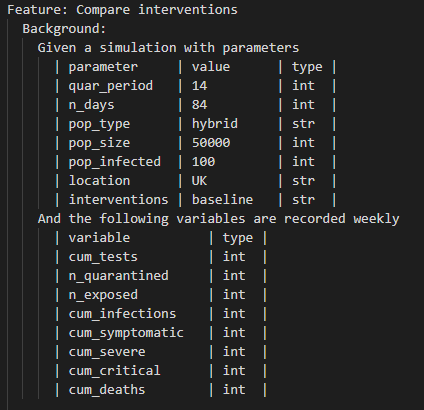
\includegraphics[width=8cm]{images/featureFile.png}\\
Figure 1. A feature file example
\end{center}
With these tests written, behave can reading the input parameters, put the inputs into the system the produce the results, and record the results. By verify these results, tester then can see if the system has any error. 
\subsection{Cucumber}
When test case is written, it requires a tool to read its specifications and see if the system works as the test-case specify. Cucumber is the tool that developed for this purpose, it read specifications written in plain text with a certain format and validate if the software does what those specifications say [11] and create a report. For cucumber to understand the specifications, it must be written in gherkin language, gherkin uses a set of grammar and special keywords to give plain text structure so that cucumber could understand it, one of the pros for gherkin is that keyword can be translated to other languages, making it usable for people who don’t speak English [12]. A proper gherkin grammar starts by giving a context, then describe an event, and after that what should happen after the event. With these grammars, tester can specify a situation in the system, describe a certain parameter, and what the results should be with those parameters.
\subsection{Casual testing and its problem}
With the help of behave and cucumber, we have the ability to test computational models, it is possible to test the entire system, but it will take to much time since computational models are usually in big scale. This is when causal model can help simplify the testing process. Causal model is a way to represent causal relationship within a system through mathematical model. It helps tester monitor causal relationship in the data [13]. A causal module can predict the behavior of a system, by comparing different inputs and the outputs a system produces, it can explore the cause and influence of a certain relationship [14]. By understand these relationships, tester can test parts of the system by see if the inputs and outputs follow the same behaviour. This can reduce the time required to test a complicate system by only test parts of it, then combine the results, and testers can have a full picture of how the system perform. This is unlike the tradition method, where it requires to test the entire system all at once, and may require lots of time if it is a complicate system.\\*
Causal testing can be a really useful testing method for software engineer [15], but for people who are not a software engineer, this could be a difficult method to use. Tester who wants to use causal model as a way to test system needs to have prior knowledge in how variables work in a software, this mean people who may not have that much knowledge in software engineering, for example researchers in other field, might not be able to conduct this method of testing in their software. 


\section{Summary}

Behave is a powerful testing tool for software tester’s, based on the behavior-driven development method, encourage people who are not specialize in software engineering to take part in testing. Assist by cucumber, a tool where user can describe testing steps in an easy-to-understand manner, and cucumber compile and produce the results. With causal model, tester can effectively test large and complex computational models, saving time by only test parts of the system one at a time and combine the result together. But the problem is that when using causal model testing, its is inaccessible for most people, due to its lack of user-friendly function. In order to make it more user friendly, we can integrate cucumber and behave with it to make it where user can use causal model testing by using behave and cucumber specify the testing process.
